%%%%%%%%%%%%%%%%%%%%%%%%%%%%%%%%%%%%%%%%%%%%%%%%%%%%%%%%%%%%%%%%%%%%%%
%
% Dario Palminio
%
% LaTeX Template: Curriculum Vitae
%
% Source: http://www.howtotex.com/
% Feel free to distribute this template, but please keep the
% referal to HowToTeX.com.
% Date: July 2011
% 
%%%%%%%%%%%%%%%%%%%%%%%%%%%%%%%%%%%%%%%%%%%%%%%%%%%%%%%%%%%%%%%%%%%%%%
% How to use writeLaTeX: 
%
% You edit the source code here on the left, and the preview on the
% right shows you the result within a few seconds.
%
% Bookmark this page and share the URL with your co-authors. They can
% edit at the same time!
%
% You can upload figures, bibliographies, custom classes and
% styles using the files menu.
%
% If you're new to LaTeX, the wikibook is a great place to start:
% http://en.wikibooks.org/wiki/LaTeX
%
%%%%%%%%%%%%%%%%%%%%%%%%%%%%%%%%%%%%%%%%%%%%%%%%%%%%%%%%%%%%%%%%%%%%%%
\documentclass[paper=a4,fontsize=11pt]{scrartcl} % KOMA-article class
							
\usepackage[english]{babel}
\usepackage[utf8x]{inputenc}
\usepackage[protrusion=true,expansion=true]{microtype}
\usepackage{amsmath,amsfonts,amsthm}     % Math packages
\usepackage{graphicx}                    % Enable pdflatex
\usepackage[svgnames]{xcolor}            % Colors by their 'svgnames'
\usepackage{geometry}
	\textheight=700px                    % Saving trees ;-)
\usepackage{url}

\frenchspacing              % Better looking spacings after periods
\pagestyle{empty}           % No pagenumbers/headers/footers

%%% Custom sectioning (sectsty package)
%%% ------------------------------------------------------------
\usepackage{sectsty}

\sectionfont{%			            % Change font of \section command
	\usefont{OT1}{phv}{b}{n}%		% bch-b-n: CharterBT-Bold font
	\sectionrule{0pt}{0pt}{-5pt}{3pt}}

%%% Macros
%%% ------------------------------------------------------------
\newlength{\spacebox}
\settowidth{\spacebox}{8888888888}			% Box to align text
\newcommand{\sepspace}{\vspace*{1em}}		% Vertical space macro

\newcommand{\MyName}[1]{ % Name
		\Huge \usefont{OT1}{phv}{b}{n} \hfill #1
		\par \normalsize \normalfont}
		
\newcommand{\MySlogan}[1]{ % Slogan (optional)
		\large \usefont{OT1}{phv}{m}{n}\hfill \textit{#1}
		\par \normalsize \normalfont}

\newcommand{\NewPart}[1]{\section*{\uppercase{#1}}}

\newcommand{\PersonalEntry}[2]{
		\noindent\hangindent=2em\hangafter=0 % Indentation
		\parbox{\spacebox}{        % Box to align text
		\textit{#1}}		       % Entry name (birth, address, etc.)
		\hspace{1.5em} #2 \par}    % Entry value

\newcommand{\SkillsEntry}[2]{      % Same as \PersonalEntry
		\noindent\hangindent=2em\hangafter=0 % Indentation
		\parbox{\spacebox}{        % Box to align text
		\textit{#1}}			   % Entry name (birth, address, etc.)
		\hspace{1.5em} #2 \par}    % Entry value	
		
\newcommand{\EducationEntry}[4]{
		\noindent \textbf{#1} \hfill      % Study
		\colorbox{Black}{%
			\parbox{6em}{%
			\hfill\color{White}#2}} \par  % Duration
		\noindent \textit{#3} \par        % School
		\noindent\hangindent=2em\hangafter=0 \small #4 % Description
		\normalsize \par}

\newcommand{\WorkEntry}[4]{				  % Same as \EducationEntry
		\noindent \textbf{#1} \hfill      % Jobname
		\colorbox{Black}{\color{White}#2} \par  % Duration
		\noindent \textit{#3} \par              % Company
		\noindent\hangindent=2em\hangafter=0 \small #4 % Description
		\normalsize \par}

%%% Begin Document
%%% ------------------------------------------------------------
\begin{document}
% you can upload a photo and include it here...
%\begin{wrapfigure}{l}{0.5\textwidth}
%	\vspace*{-2em}
%		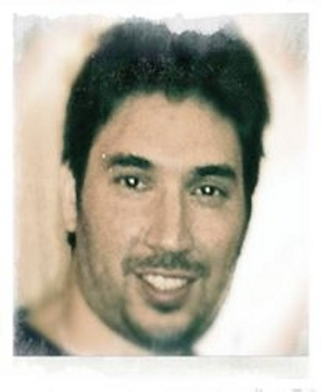
\includegraphics[width=0.15\textwidth]{photo}
%\end{wrapfigure}

\begin{figure}
	\hfill
	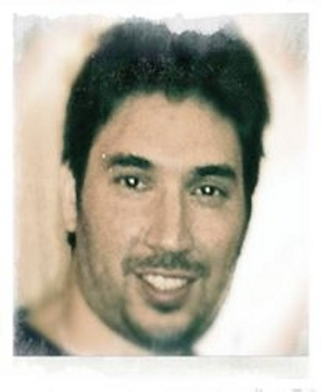
\includegraphics[width=0.2\textwidth]{photo}
	\vspace{-7cm}
\end{figure}

\MyName{Dario Palminio}
\MySlogan{Curriculum Vitae}

\sepspace

%%% Personal details
%%% ------------------------------------------------------------
\NewPart{Personal details}{}

\PersonalEntry{Birth}{January 6, 1977}
\PersonalEntry{Address}{5000 Cordoba, Argentina}
\PersonalEntry{Phone}{(000) 000-0000}
\PersonalEntry{Mail}{\url{dario.palminio@gmail.com}}
\PersonalEntry{Website}{\url{https://www.palminio.com}}
\PersonalEntry{linkedin}{\url{https://www.linkedin.com}}

%%% Education
%%% ------------------------------------------------------------
\NewPart{Education}{}

%2003 - Systems Engineer: School of Exact Sciences, UNPA-UACO National University. Graduated in 2003.
\EducationEntry{Systems Engineer}{2003}{UNPA-UACO National University}{Systems Engineer: School of Exact Sciences, UNPA-UACO National University. Graduated in 2003.}
\sepspace

%2000, Analyst: University Analyst Programmer: School of Engineering, UNPSJB University National. Graduated in 2000.
\EducationEntry{Analyst}{2000}{UNPSJB University National}{Analyst: University Analyst Programmer: School of Engineering, UNPSJB University National. Graduated in 2000.}
\sepspace

%1995, Electromechanical: Electromechanical technician: School ENET 1. Graduated in 1995.
\EducationEntry{Electromechanical}{1995}{School ENET 1}{Electromechanical: Electromechanical technician: School ENET 1. Graduated in 1995.}
\sepspace

%%% Work experience
%%% ------------------------------------------------------------
\NewPart{Work experience}{}

%2014-2015 Globant (globant.com) Software Engineer.
\EducationEntry{Globant}{2015-present}{Technical Leader, Focal point and Java developer}
{Technical Lead on Perl/Java Technologies in a context of LAN airline at Globant Company. The Perl Technologies used was Perl (POO with Moose, cgi, Test::Moore, Template Toolkit), MySQL, Linux, SVN, Git-Svn, CSS3, HTML5, Eclipse (RSE, EPIC), Review Board, Jenkins, etc. The Java Technologies used was SOAP, RESTful/RESTEasy, Spring, Maven, Javascript with front-end using MVC (Backbone.js). Project related to data collection from web site to send to Google Analytic.}
\sepspace

%2012-2014 IBA Entertainment limited as Software Engineer Freelancer.
\EducationEntry{IBA Entertainment limited}{2012-2014}{Software Engineer Freelancer}
{Software Engineer (as Contractor Freelancer) on Perl Technologies in a context of sportsbetting (Bet3000.com). Some technologies: Perl 5, EmbPerl Object, Object Perl, JSON, RESTful, Mojolicious, Perl DBI. Development in Bet3000 Project (www.bet3000.com) to International Betting Association.}
\sepspace

%2013-2014 Make IT Coop. As Associate, Secretary
\EducationEntry{Make IT Coop.}{2013-2014}{Associate, Secretary}{
Software Engineer}
\sepspace

%2008-2010 Motorola Mobility as Software Engineer.
\EducationEntry{Motorola Mobility}{2008-2010}{Software Engineer}
{Software Engineering on Java Technologies (J2EE in a context of telecommunications mobile devices) at Motorola Mobility of Argentina S.A.}
\sepspace

%2008-2010 Motorola S.C.A (Contractor Vates) as Software Engineer.
\EducationEntry{Motorola S.C.A (Contractor Vates)}{2008-2010}{Software Engineer}
{Java development (J2SE and J2EE in a context of telecommunications mobile devices)}
\sepspace

%2008 Vates (www.vates.com) as Systems Engineer.
\EducationEntry{Vates}{2008}{Systems Engineer}
{Java Developer in context of system business process management.}
\sepspace

%2007 Santex America S.A. (santexgroup.com) as Software Engineer: Java Developer.
\EducationEntry{Santex America S.A.}{2007}{Software Engineer, Java Developer}
{1) Java Developer in context of system business process management. 2) Instructor of "Oracle 9i: Build J2EE Applications" at InMotion, Santiago de Chile (Chile);
3) Instructor of "Oracle AS 10g: R3 Build J2EE Applications" at Oracle, Buenos Aires (Arg.).}
\sepspace

%2007 AYI & Asociados (BADI S.R.L) as Software Engineer: Java Developer, Computer Consultant Java.
\EducationEntry{AYI and Asociados (BADI S.R.L)}{2007}{Software Engineer, Java Developer, Computer Consultant Java}
{Oracle Java Developer (J2EE) in context of credit card company (Tarjeta Naranja).}
\sepspace

%2006 Informatic forensics – Tribunal third in Comodoro Rivadavia City: Informatic Forensics.
\EducationEntry{Tribunal third in Comodoro Rivadavia}{2006}{Informatic forensics}{
Tribunal third in Comodoro Rivadavia City: Informatic Forensics}
\sepspace

%2004-2006 24 months in Municipality of Comodoro Rivadavia city, Systems Engineer Juridical Informatics, Technical Leader.
\EducationEntry{Municipality of Comodoro Rivadavia}{2004-2006}{Systems Engineer Juridical Informatics, Technical Leader}
{Technical lead at Digesto Project (and VB Developer and PHP Developer) in context of legal area (Asesoría letrada) of a town hall (Municipality).}
\sepspace

%2004-2005 Teacher Mathematic Teacher, Software Teacher, Computation Teacher.
\EducationEntry{Teacher}{2004-2005}{Teacher Mathematic Teacher, Software Teacher, Computation Teacher}
{Profesor de Informática: 1- Computation Teacher I (Basic Informatic) - ISIS (Private Institute Third); 2- Computation Teacher II (Software Applications) - ISIS (Private Institute Third); 3- Computation Teacher III (Linux and Windows Net) - ISIS (Private Institute Third); Profesor de Software y Matemática (Mathematics and Software Teacher): 1- Course, Software Teacher: Adaptación al ambiente de trabajo en ENET 2 (technical school); 2- Course, Mathematic Teacher of 8-EGB  (two grades)- School 119 (C. R.); 3- Course, Mathematic Teacher of 9-EGB (two grades)- School 119 (C. R.).
}
\sepspace

%2000-2003 - DeSoft Development of Software
\EducationEntry{DeSoft}{2000-2003}{Developer, Technical Leader}{
Developer, Technical Leader}
\sepspace

%%% Skills
%%% ------------------------------------------------------------
\NewPart{Skills}{}

\SkillsEntry{Languages}{Spanish (mother tongue)}
\SkillsEntry{}{English (level 2)}


\SkillsEntry{Software}{
\textsc{Java}, \LaTeX, \textsc{Perl}, \textsc{MySQL}
}


%%% References
%%% ------------------------------------------------------------
\NewPart{References}{}
Available upon request
\end{document}
